%\documentclass[12pt]{scrreprt}
\documentclass[12pt]{report} 
% language may be romanian or english (default is english)
% type may be bachelor or master (default is bachelor)
\usepackage[language=romanian, type=bachelor]{style}

%\geometry{a4paper,top=2.5cm,left=3cm,right=2.5cm,bottom=2.5cm}
%in style
%controlling the appearance of your headers and footers
\usepackage{fancyhdr}
\pagestyle{fancy}
\setlength{\headheight}{16pt}
\lhead{}
\chead{}
\renewcommand{\headrulewidth}{0.2pt}
\renewcommand{\footrulewidth}{0.2pt}

\begin{document}

\specialization{INFORMATICĂ ROMÂNĂ}
\title{Aplicabilitatea modelelor AI de estimare a adâncimii monocular în detecția și evitarea obstacolelor}
\author{Ștefan - Lucian Grămadă}
\supervisor{Prof. Dr. Laura Silvia Dioșan \\ drd. Alexandru Manole}
\titleeng{Applicability of monocular depth estimation AI models in obstacle detection and avoidance}

\maketitle
\maketitleeng


% \newpage
% \thispagestyle{empty}
% \mbox{}
\newpage
\pagenumbering{roman} 

\cleardoublepage
ABSTRACT
\vspace{0.5cm}	
\hrule
\vspace{0.5cm}	
%\cleardoublepage

% Abstract: un rezumat în limba engleză cu prezentarea, pe scurt, a conținutului pe capitole, punând accent pe contribuțiile proprii și originalitate

This thesis presents the design and implementation of an assistive system for visually impaired people, intended to facilitate independent navigation through obstacle avoidance, with a focus on an optimal balance between accuracy and financial accessibility. The motivation stems from the need to provide a capable technological solution at a reduced cost, thereby enabling access on a large scale. The proposed implementation uses a Raspberry Pi 5 (8GB) together with the AI HAT+ hardware accelerator, a configuration that runs a monocular Depth Anything V2 model capable of estimating depth from a video stream captured by a single camera.

The principal contribution is a system built from scratch that replaces specialized depth-sensing hardware (stereo cameras or LiDAR) with a monocular depth-estimation model: from the depth map it detects the ground plane using the classical RANSAC algorithm and plans a minimum-cost route with the A* pathfinding algorithm. The system was first developed on a laptop with a dedicated NVIDIA RTX 5070 Ti Mobile GPU, which enabled a more capable model, Depth Anything 3 Metric - Large, and was then ported to the Raspberry Pi.

On both platforms the system runs at roughly 11--13 frames per second (under 150 ms per frame on average). Depth estimation is consistent on the laptop, but on the Raspberry Pi, the smaller previous-generation model yields less detailed depth that degrades ground detection, and the pathfinding stage becomes the bottleneck in complex scenes. The work concludes that depth-estimation quality, conditioned by the hardware, is the decisive performance factor, and points to semantic ground segmentation and multi-view 3D reconstruction as future directions.

\tableofcontents


\newpage
\pagenumbering{arabic}

\chapter{Introducere}

%\chapter*{Introducere}
\label{intro}

\par Conform raportului oficial al Organizației Mondiale a Sănătății \cite{who2019}, aproximativ 2,2 miliarde de oameni trăiesc cu o formă de deficiență de vedere, dintre care cel puțin 1 miliard au o deficiență care ar fi putut fi prevenită sau care nu a fost încă tratată. Impactul funcțional este cel mai sever în rândul celor 43,3 milioane de persoane care suferă de orbire totală și al celor 295 de milioane cu deficiențe moderate până la severe (MSVI) \cite{vleg2021}. Din perspectivă clinică, nevoia de asistență pentru deplasare devine universală odată ce acuitatea vizuală scade sub pragul de $3/60$.

În ceea ce privește mecanismele de sprijin, deși utilizarea câinilor-ghid este considerată în literatura de reabilitare drept reperul pentru fluiditatea mișcării, accesul global rămâne extrem de scăzut. Datele furnizate de International Guide Dog Federation \cite{igdf2023} relevă existența a doar aproximativ 30.000 de câini activi la nivel mondial, ceea ce înseamnă că mai puțin de 0,1\% din populația care ar avea nevoie clinică de un astfel de sprijin beneficiază efectiv de el. Această disparitate este accentuată de barierele economice, costul de antrenament al unui singur exemplar fiind estimat între 40.000\$ și 60.000\$ \cite{cost2018}. În acest context, majoritatea persoanelor cu deficiențe de vedere rămân dependente fie de bastonul alb (utilizat de aproximativ 33,8\% din populația vizată), fie de asistența umană directă \cite{nature2021}.

O evoluție tehnologică recentă, cu un impact semnificativ asupra pieței dispozitivelor portabile (\textit{wearable technology}), este reprezentată de ascensiunea ochelarilor inteligenți (\textit{Smart Glasses}) \ref{fig:figures/aria-gen-2-specs.png}. Această categorie de dispozitive a fost popularizată recent prin parteneriate strategice, precum cel dintre Meta și Ray-Ban \cite{metarayban}, care au integrat senzori optici performanți în accesorii de uz cotidian. Din punct de vedere tehnic, prezența camerei video pe aceste dispozitive permite captarea și procesarea fluxului vizual în timp real, oferind astfel o platformă potențială pentru sisteme de asistență computațională.

\begin{figure}[htbp]
    \centering
    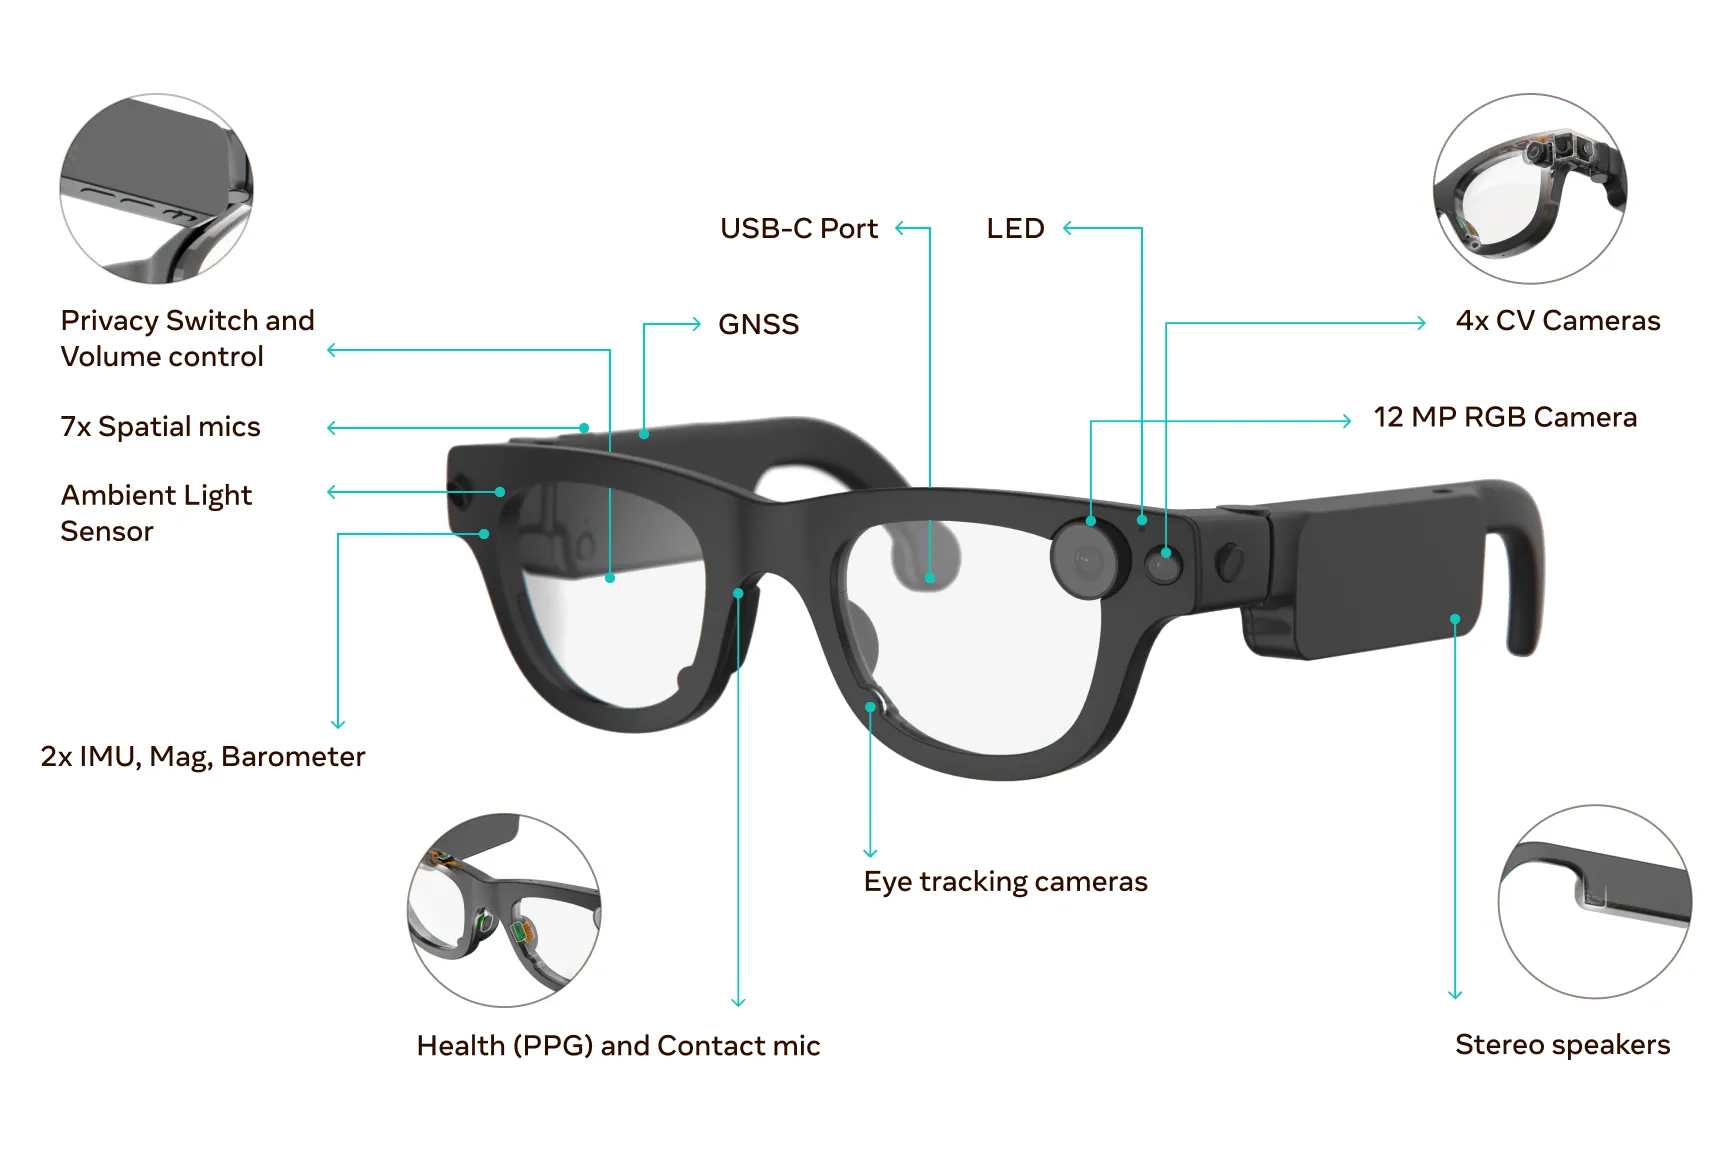
\includegraphics[width=0.7\linewidth]{figures/aria-gen-2-specs.png}
    \caption{Exemplu de dispozitiv de tip Smart Glasses, Aria Gen 2. Sursă: \href{https://roadtovrlive-5ea0.kxcdn.com/wp-content/uploads/2025/06/aria-gen2.jpg}{Road to VR}}
    \label{fig:figures/aria-gen-2-specs.png}
\end{figure}

Cu toate acestea, deși ochelarii Ray-Ban Meta oferă funcționalități AI impresionante, precum recunoașterea obiectelor și a scenelor din jur, traducerea în timp real, identificarea textului din mediul înconjurător și asistentul vocal integrat bazat pe Meta AI \cite{metarayban}, această tehnologie puternică rămâne limitată în privința utilității pentru persoanele cu deficiențe de vedere. Cea mai utilizată aplicație dedicată acestui segment al populației este Be My Eyes \cite{bemyeyes}, o platformă care conectează utilizatorii nevăzători cu voluntari ce le oferă asistență vizuală în timp real prin intermediul camerei telefonului. Limitarea fundamentală a acestei soluții constă în dependența de disponibilitatea voluntarilor umani, ceea ce o face inadecvată pentru scenarii de navigație autonomă continuă sau pentru situații în care intervenția imediată este esențială.

În acest context considerăm că hardware-ul existent și inovațiile recente din domeniul inteligenței artificiale ar permite dezvoltarea de aplicații care să permită persoanelor cu deficiente de vedere, o independență mult mai ridicată care nu se bazează pe ghizi canini.

Motivată de nevoia critică de independență a persoanelor cu deficiențe severe de vedere și valorificând accesibilitatea actuală a tehnologiei de tip \textit{Smart Glasses}, prezenta lucrare propune dezvoltarea unui sistem compact și eficient din punct de vedere al costurilor. Obiectivul principal al sistemului este de a sprijini utilizatorul în detectarea și evitarea obstacolelor, facilitând astfel o mobilitate mai sigură și mai autonomă.

Lucrarea de față abordează tocmai acest gol: investigarea și implementarea unui sistem de detecție și evitare a obstacolelor destinat persoanelor cu deficiențe de vedere, construit pe o platformă accesibilă din punct de vedere financiar, în special Raspberry Pi \cite{raspberrypi5}. Procesul de dezvoltare a debutat pe o platformă de tip x86 echipată cu o unitate de procesare grafică dedicată, urmând ca soluția să fie ulterior portată pe platforma țintă. Această strategie de dezvoltare în două etape a condus la diferențe măsurabile de performanță între cele două configurații hardware, diferențe datorate în principal capacității de procesare superioare oferite de GPU-ul dedicat. Din acest motiv, pe parcursul lucrării ambele platforme sunt analizate comparativ, iar rezultatele obținute pe fiecare sunt prezentate în paralel. Deși platforma țintă rămâne Raspberry Pi, rezultatele superioare înregistrate pe platforma de dezvoltare sunt incluse ca referință pentru a ilustra potențialul maxim al algoritmilor propuși.

Structura lucrării este organizată după cum urmează: Capitolul~\ref{chap:ch2} trece în revistă literatura de specialitate ce a stat la baza creionării sistemului descris în lucrare. Ulterior, în Capitolul~\ref{chap:ch3} este prezentată metodologia de dezvoltare și sunt analizate dificultățile tehnice întâmpinate. Capitolul~\ref{chap:ch4} descrie arhitectura aplicației propuse. În Capitolul~\ref{chap:ch5} sunt prezentate și discutate performanțele obținute pe cele două platforme hardware. În final, Capitolul~\ref{conclusions} sintetizează concluziile lucrării și propune direcții viitoare de cercetare.

\section{Utilizarea instrumentelor IA generative}
\label{sec:ai_usage}

În timpul elaborării acestei lucrări, autorul a folosit Claude Opus 4.8 pentru a găsi erori în codul sursă, a refactoriza fișiere de cod, și pentru a reformula porțiuni din prezenta lucrare. După utilizarea acestui instrument/serviciu, autorul a revizuit și editat conținutul generat și își asumă întreaga responsabilitate pentru conținutul lucrării.

%\addcontentsline{toc}{chapter}{Introducere}
%\addcontentsline{toc}{chapter}{Introduction}

\chapter{Lucrări Conexe}
\label{chap:ch2}

\par Acest capitol prezintă lucrările și metodele pe care se bazează soluția propusă. Sunt discutate, în ordine, calibrarea camerelor și corectarea distorsiunilor optice, metodele de estimare a adâncimii din imagini monoculare și multi-vizuale folosind modele bazate pe rețele neuronale, algoritmul RANSAC pentru filtrarea planului de mers din date ce conțin zgomot, precum și algoritmul A* pentru optimizarea traiectoriilor. Fiecare secțiune descrie principiile de funcționare ale metodelor relevante și modul în care acestea sunt utilizate sau adaptate în cadrul lucrării de față.

\section{Calibrarea Camerelor și Anularea Distorsiunilor}
\label{sec:ch2sec1}

\par Fundamentul oricărei analize metrice dintr-o imagine este stabilit prin calibrarea camerei. În lucrarea sa de referință \cite{zhang2000}, Zhang propune o tehnică flexibilă care a democratizat accesul la viziunea 3D prin eliminarea necesității unor aparate de calibrare costisitoare. Autorul demonstrează că utilizarea unui model plan (checkerboard) \ref{fig:figures/calib.io_checker_200x150_8x11_15.pdf} observat din cel puțin două orientări diferite este suficientă pentru a determina parametrii intrinseci și extrinseci ai camerei. Metoda se bazează pe calculul homografiei între planul modelului și proiecția sa în imagine, urmată de o rafinare neliniară prin criteriul verosimilității maxime care ia în considerare și distorsiunile radiale ale lentilei. Această abordare a transformat calibrarea dintr-un proces restrictiv de laborator într-o procedură aplicabilă în scenarii de utilizare reală.

\begin{figure}[htbp]
    \centering
    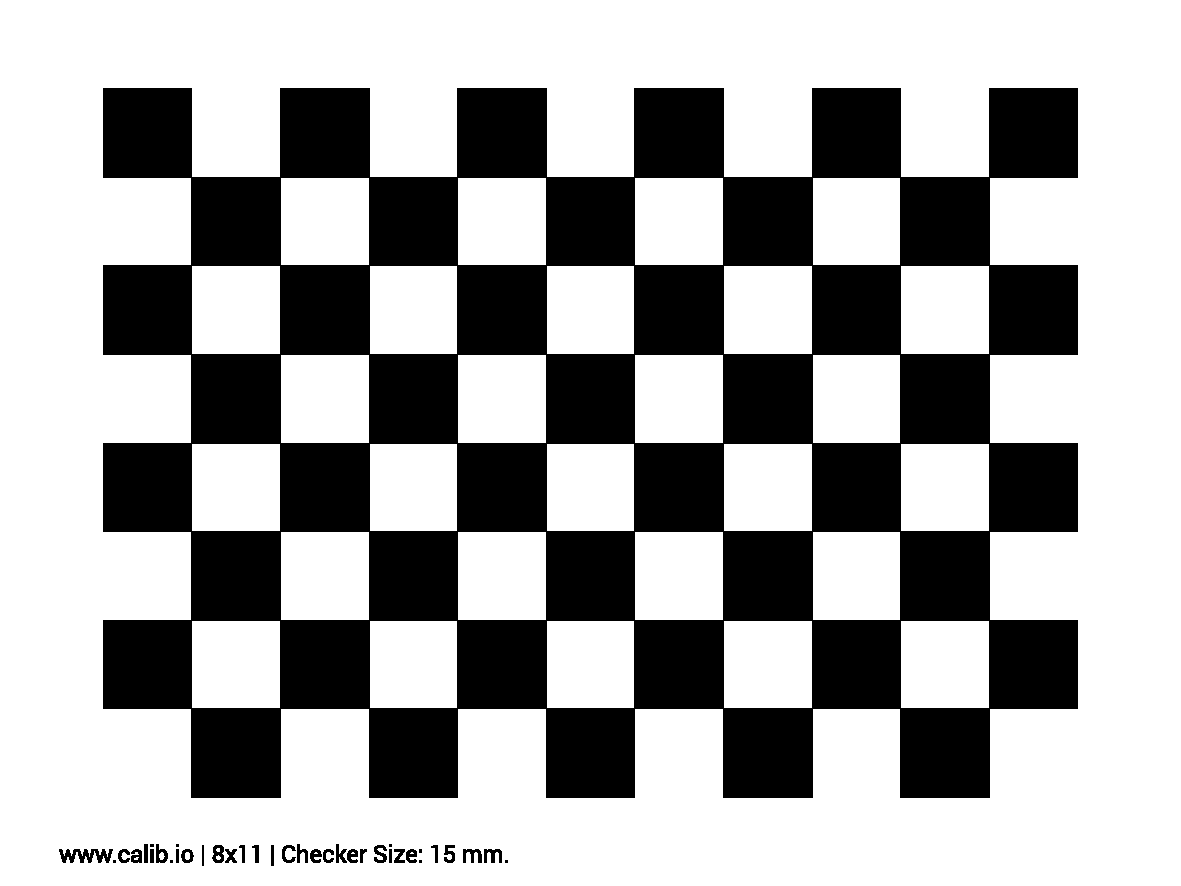
\includegraphics[width=0.8\linewidth]{figures/calib.io_checker_200x150_8x11_15.pdf}
    \caption{Exemplu de checkerboard pattern utilizat pentru a efectua calibrarea camerei, având 8 linii, 11 coloane(6 linii interne, 9 coloane interne) în care fiecare latură a unui pătrat măsoară 15 milimetrii pe o suprafață plană dreptunghiulară cu lungimea de 200 milimetrii, și lățimea de 150 de milimetrii, generat de platforma \url{https://calib.io}.}
    \label{fig:figures/calib.io_checker_200x150_8x11_15.pdf}
\end{figure}

Calibrarea estimează matricea $\mathbf{A}$ și coeficienții de distorsiune radială prin minimizarea erorii de reproiecție pe un set de imagini ale unui șablon de tip tablă de șah cu dimensiuni cunoscute. Soluția constă dintr-o estimare inițială în formă închisă, rafinată ulterior prin algoritmul Levenberg-Marquardt \cite{zhang2000}.

Parametrii obținuți sunt utilizați în două etape ale procesării. În primul rând, fiecare cadru este rectificat geometric pentru a elimina distorsiunile radiale ale obiectivului, asigurând consistența cu modelul pinhole \cite{hartley2004}. În al doilea rând, lungimea focală medie $f = (\alpha +
\beta)/2$ este utilizată pentru conversia ieșirii modelului de adâncime în metri, conform formulei \cite{depthanything3}:

\begin{equation}
    d_{\text{metric}} = \frac{f \cdot d_{\text{raw}}}{300}
\end{equation}

unde $d_{\text{raw}}$ reprezintă valoarea brută estimată de model, iar constanta $300$ provine din transformarea spațiului canonic al camerei utilizată în antrenarea modelului \cite{depthanything3}. În absența calibrării, lungimea focală este estimată presupunând un câmp vizual orizontal de $70°$, permițând funcționarea sistemului cu o precizie metrică redusă.

\section{Modele AI pentru Estimarea Adancimilor}
\label{sec:ch2sec2}

\par Odată stabilit modelul geometric, sarcina centrală devine inferarea adâncimii din imagini monoculare. Evoluția acestei sarcini este urmărită cel mai bine prin familia de modele \emph{Depth Anything}, prezentată în continuare în ordine cronologică.

\par Punctul de plecare îl reprezintă Depth Anything V1, introdus de Yang et al. \cite{yang2024depthv1} în cadrul conferinței Computer Vision and Pattern Recognition (CVPR) din 2024. Contribuția centrală a acestei lucrări nu constă într-un modul arhitectural nou, ci în scalarea masivă a datelor de antrenament: autorii proiectează un motor de date (\emph{data engine}) care colectează și etichetează automat aproximativ 62 de milioane de imagini neetichetate, alături de cele 1{,}5 milioane de imagini etichetate disponibile. Din punct de vedere arhitectural, modelul combină un encoder de tip DINOv2 \cite{oquab2024dinov2} cu un decodor DPT și estimează adâncime relativă de tip afin-invariant. Pentru ca volumul mare de date să fie valorificat, sunt propuse două strategii: impunerea unui obiectiv de optimizare mai dificil prin augmentări puternice, care forțează modelul să caute activ indicii vizuale suplimentare, și o supraveghere auxiliară care transferă priorii semantici bogați din encoderul preantrenat. Rezultatul este un model fundațional cu o capacitate de generalizare \emph{zero-shot} remarcabilă pe imagini din medii necunoscute, putând fi rafinat ulterior pentru adâncime metrică pe seturi precum NYUv2 \cite{silberman2012nyuv2} și KITTI \cite{geiger2012kitti}.

\par Construind direct peste acest fundament, Yang et al. \cite{yang2024depth} introduc Depth Anything V2, care schimbă sursa principală a supervizării: în locul imaginilor reale etichetate manual, antrenarea se bazează pe date sintetice, ale căror etichete de adâncime sunt absolut precise și permit învățarea detaliilor geometrice fine. Pentru a depăși decalajul de domeniu dintre imaginile sintetice și cele reale, V2 păstrează ideea scalării datelor din V1, dar o reorganizează într-o schemă de tip profesor-elev (\emph{teacher-student}): un model profesor de mare capacitate, antrenat exclusiv pe date sintetice, generează etichete pseudo-adâncime pe un volum masiv de imagini reale neetichetate, pe care apoi sunt antrenate modelele-elev. Față de V1, această modificare aduce hărți de adâncime mai robuste și cu o granularitate net superioară, în special în zonele cu structuri fine și obiecte transparente, păstrând în același timp o eficiență computațională ridicată.

Extinzând aceste capacități către o înțelegere multi-vizuală, Depth Anything 3 (DA3) \cite{depthanything3} propune o metodă de recuperare a spațiului vizual din orice număr de intrări, indiferent dacă poziția camerei este cunoscută sau nu. Contribuția majoră a DA3 constă în demonstrarea faptului că o arhitectură simplă, bazată pe un transformator standard (vanilla DINO), este suficientă pentru a obține rezultate de ultimă oră fără a fi nevoie de specializări arhitecturale complexe. Prin utilizarea unui target de predicție de tip „depth-ray”, modelul reușește o consistență spațială remarcabilă, depășind standardele anterioare în acuratețea geometrică și în estimarea poziției camerei cu peste 23\% față de predecesorii săi.

\par Pentru a sintetiza evoluția celor trei generații, Tabelul~\ref{tab:da_params} compară dimensiunea modelelor, iar Tabelul~\ref{tab:da_perf} rezumă performanța în estimarea adâncimii relative (zero-shot) și metrice. La nivel de capacitate, se observă că abia V2 introduce varianta uriașă (\emph{Giant}, $\sim$1,3 miliarde de parametri), folosită ca model profesor, în timp ce DA3 menține aceeași gamă de dimensiuni, dar cu un backbone ușor mai compact. În privința metricilor clasice de adâncime, valorile sunt aproape identice între V1 și V2: progresul real al V2 se manifestă în detaliile fine și robustețe, aspecte care, așa cum notează chiar autorii \cite{yang2024depth}, nu sunt surprinse de aceste benchmark-uri standard. DA3 \cite{depthanything3} aduce câștiguri vizibile mai ales pe seturi precum ETH3D și își concentrează evaluarea pe acuratețea geometrică și pe estimarea poziției camerei, motiv pentru care nu raportează rezultate metrice monoculare în același format ca predecesorii.

\begin{table}[htbp]
    \centering
    \begin{tabular}{lccc}
        \toprule
        Variantă (encoder) & V1 & V2 & DA3 \\
        \midrule
        Small (ViT-S) & 24,8M & 24,8M & 22M \\
        Base (ViT-B)  & 97,5M & 97,5M & 86M \\
        Large (ViT-L) & 335,3M & 335,3M & 300M \\
        Giant (ViT-g) & --- & 1,3B & 1,13B \\
        \bottomrule
    \end{tabular}
    \caption{Numărul de parametri pentru variantele celor trei generații \emph{Depth Anything} \cite{yang2024depthv1, yang2024depth, depthanything3}. \emph{Notă:} pentru V1 și V2 cifrele provin din depozitele oficiale și includ modelul complet (encoder DINOv2 + decodor DPT), în timp ce pentru DA3 valorile raportate corespund în principal backbone-ului DINOv2; numerele nu sunt, prin urmare, măsurate identic.}
    \label{tab:da_params}
\end{table}

\begin{table}[htbp]
    \centering
    \begin{tabular}{lccccc}
        \toprule
         & \multicolumn{2}{c}{V1} & \multicolumn{2}{c}{V2} & DA3 \\
        \cmidrule(lr){2-3}\cmidrule(lr){4-5}\cmidrule(lr){6-6}
        Set de date & AbsRel$\downarrow$ & $\delta_1\uparrow$ & AbsRel$\downarrow$ & $\delta_1\uparrow$ & $\delta_1\uparrow$ \\
        \midrule
        \multicolumn{6}{l}{\textit{Estimare relativă (zero-shot)}} \\
        KITTI  & 0,076 & 0,947 & 0,074 & 0,946 & 0,953 \\
        NYU    & 0,043 & 0,981 & 0,045 & 0,979 & 0,974 \\
        Sintel & 0,458 & 0,760 & 0,487 & 0,752 & 0,755 \\
        ETH3D  & 0,127 & 0,882 & 0,131 & 0,865 & 0,986 \\
        DIODE  & 0,066 & 0,952 & 0,066 & 0,952 & 0,954 \\
        \midrule
        \multicolumn{6}{l}{\textit{Estimare metrică (fine-tuned)}} \\
        NYUv2  & 0,056 & 0,984 & 0,056 & 0,984 & --- \\
        KITTI  & 0,046 & 0,982 & 0,045 & 0,983 & --- \\
        \bottomrule
    \end{tabular}
    \caption{Performanța în estimarea adâncimii (encoder ViT-L), AbsRel ($\downarrow$, mai mic e mai bun) și $\delta_1$ ($\uparrow$, mai mare e mai bun). Rezultatele V1/V2 provin din \cite{yang2024depthv1, yang2024depth}, iar coloana $\delta_1$ pentru DA3 din \cite{depthanything3} (Tabel~4, reevaluare monoculară). \emph{Notă:} DA3 raportează doar $\delta_1$ pentru adâncimea relativă și nu publică rezultate metrice monoculare în acest format, de unde marcajul „---”.}
    \label{tab:da_perf}
\end{table}

\section{Filtrarea Planului de Mers}
\label{sec:ch2sec3}

\par În procesarea datelor extrase din mediul vizual, prezența zgomotului și a erorilor sistematice este inevitabilă. Fischler și Bolles \cite{10.1145/358669.358692} au introdus algoritmul RANSAC (Random Sample Consensus) ca o soluție pentru potrivirea modelelor matematice pe seturi de date ce conțin un procent ridicat de erori brute (outliers). Spre deosebire de tehnicile de tip „least squares”, RANSAC utilizează un proces iterativ de selecție a unui subset minim de date pentru a genera un model candidat, verificând apoi consensul acestuia cu restul datelor. Această paradigmă este vitală în analiza imaginilor, unde detectorii de trăsături pot genera corespondențe eronate; RANSAC permite izolarea modelului corect (cum ar fi un plan sau o poziție a camerei) prin ignorarea zgomotului care nu se conformează structurii geometrice globale.

\section{Optimizarea Traiectoriilor}
\label{sec:ch2sec4}

\par În final, având o reprezentare stabilă a spațiului și a obstacolelor, problema deplasării este redusă la găsirea unui drum optim. Hart et al. \cite{4082128} au oferit baza formală pentru determinarea căilor de cost minim prin algoritmul A*. Acesta utilizează o funcție euristică pentru a ghida procesul de căutare într-un graf, evaluând fiecare nod prin suma dintre costul parcurs de la start ($g$) și costul estimat până la țintă ($h$). Autorii demonstrează că dacă euristica $h$ este admisibilă (adică nu supraestimează niciodată costul real), algoritmul A* garantează găsirea căii optime. Această cercetare a stabilit echilibrul matematic între eficiența căutării și certitudinea soluției, rămânând o piatră de temelie pentru orice sistem de navigație care operează în spații de stare complexe.

\chapter{Metodologie}
\label{chap:ch3}

\section{Arhitectura Generală}
\label{sec:ch3sec1}

\par Sistemul utilizează o cameră video pentru achiziția de date vizuale în timp real. Deoarece obiectivele camerelor introduc frecvent distorsiuni geometrice (în special spre extremitățile cadrului), este necesară o etapă preliminară de calibrare pentru rectificarea imaginilor. Parametrii de calibrare sunt stocați în sistem, astfel încât procesul nu necesită rulări repetate, deși utilizatorul poate opta pentru o nouă calibrare oricând este necesar.

După captare și rectificare, cadrul video este procesat de un model de estimare monoculară a adâncimii pentru a genera o hartă de adâncime (\textit{depth map}). Următoarea etapă constă în identificarea suprafeței de rulare. În această lucrare, algoritmul de detecție vizează exclusiv planuri orizontale, netede și continue, pe care le vom defini generic sub termenul de ,,sol''.

În final, integrând datele din harta de adâncime cu geometria planului solului, sistemul stabilește două puncte de referință în spațiul 3D proiectat. Un algoritm de planificare a traseului (\textit{pathfinding}) calculează apoi drumul de lungime minimă între aceste puncte, evitând obstacolele detectate în scenă. Fluxul logic al procesării datelor este sintetizat în diagrama \ref{fig:data_flow}.

\begin{figure}[h]
    \centering
    \begin{tikzpicture}[node distance=2cm]

        % --- Fluxul Principal ---

        % Pas 1: Input
        \node (input) [io] {Captură Video (Real-time)};

        % Pas 2: Calibrare
        \node (calib) [process, below of=input] {Calibrare și Rectificare \\ (Corecție Distorsiune)};

        % Pas 3: Depth Estimation
        \node (depth) [process, below of=calib, yshift=-0.5cm] {Estimare Monoculară \\ a Adâncimii};

        % Pas 4: Ground Detection
        \node (ground) [process, below of=depth] {Detecția Suprafeței \\ (Planul Pământului)};

        % Pas 5: Pathfinding
        \node (path) [process, below of=ground] {Algoritm Pathfinding \\ (Drum Minim)};

        % Pas 6: Output
        \node (output) [io, below of=path] {Sistem de Ocolire Obstacole};

        % --- Elemente Auxiliare (Logica de Calibrare) ---

        % Storage pentru calibrare
        \node (data) [storage, right=2cm of calib] {Date de \\ Calibrare};

        % --- Săgeți și Conexiuni ---

        \draw [arrow] (input) -- (calib);
        \draw [arrow] (calib) -- (depth);
        \draw [arrow] (depth) -- (ground);
        \draw [arrow] (ground) -- (path);
        \draw [arrow] (path) -- (output);

        % Fluxul de date pentru calibrare (bidirecțional conform descrierii tale)
        \draw [arrow, <->, dashed] (calib) -- (data);

        % Adnotare pentru calibrare
        \node [right=0.2cm of data, text width=3cm, font=\footnotesize\itshape] {Salvate în sistem; pot fi actualizate la cerere.};

    \end{tikzpicture}
    \caption{Diagrama fluxului de date și a procesării în sistemul de asistență la mobilitate.}
    \label{fig:data_flow}
\end{figure}

\section{Caracteristicile Dispozitivelor Hardware Folosite}
\label{sec:ch3sec2}

\par Dezvoltarea sistemului s-a desfășurat în două etape distincte. Într-o primă fază, implementarea și testarea au fost realizate pe un laptop echipat cu placă grafică dedicată, urmând ca ulterior sistemul să fie adaptat și optimizat pentru a rula pe un dispozitiv cu resurse limitate, respectiv un Raspberry Pi în combinație cu un accelerator neuronal dedicat.

\par Laptopul utilizat este un Lenovo Legion Pro 5 16IAX10H, echipat cu un procesor Intel Core Ultra 9 275HX, cu 24 de nuclee și o frecvență maximă de 5,40 GHz \cite{intel_core_ultra9_275hx}, și o placă grafică NVIDIA GeForce RTX 5070 Ti Mobile, cu 12 GB memorie VRAM dedicată și un TDP configurabil de până la 140W.

\par Platforma embedded este reprezentată de un Raspberry Pi 5 cu 8 GB RAM \cite{raspberrypi5}, la care s-a atașat modulul Raspberry Pi AI HAT+, un accelerator neuronal cu o putere de procesare de 26 TOPS, bazat pe procesorul Hailo-8 \cite{raspberrypi_aihat}. Implicațiile acestei configurații asupra performanței sistemului, atât avantajele, cât și limitările impuse, sunt discutate în detaliu în secțiunea~\ref{sec:ch3sec4}, dedicată modelelor monoculare de estimare a adâncimii.

\section{Calibrarea Camerei}
\label{sec:ch3sec3}

\par Calibrarea camerei reprezintă un pas esențial în obținerea unor estimări metrice precise ale adâncimii, în special atunci când se utilizează un model monocular metric de estimare a adâncimii. Procesul de calibrare determină parametrii intrinseci ai camerei, distanța focală și punctul principal, precum și coeficienții de distorsiune, care modelează deformările geometrice introduse de lentilă, cel mai frecvent manifestate la marginile imaginii. Fără corectarea acestor distorsiuni, estimările de adâncime ar acumula erori ce pot afecta semnificativ precizia sistemului de evitare a obstacolelor.

\par Metoda utilizată se bazează pe tehnica de calibrare propusă de Zhang \cite{zhang2000}, implementată în biblioteca OpenCV. Aceasta presupune captarea mai multor imagini ale unui panou de calibrare cu model de tablă de șah (\textit{checkerboard}) din unghiuri și distanțe variate, permițând estimarea robustă a parametrilor camerei prin minimizarea erorii de reproiecție.

\par Algoritmul de calibrare utilizează patru parametrii configurabili: \texttt{cols}, \texttt{rows}, \texttt{square\_mm} și \texttt{min\_frames}. Parametrii \texttt{cols} și \texttt{rows} definesc numărul de colțuri interioare detectabile ale tablei de șah pe orizontală, respectiv verticală. Parametrul \texttt{square\_mm} specifică dimensiunea reală a laturii unui pătrat, exprimată în milimetri, valoare necesară pentru a stabili corespondența dintre coordonatele din spațiul real și cele din planul imaginii. În fine, \texttt{min\_frames} indică numărul minim de cadre ce trebuie captate pentru ca estimarea parametrilor să fie suficient de stabilă. Toți acești parametrii pot fi ajustați din secțiunea \textit{Settings} a aplicației, oferind flexibilitate în funcție de camera utilizată.

\par Din punct de vedere tehnic, pentru fiecare cadru în care panoul de calibrare este detectat, algoritmul rafinează pozițiile colțurilor detectate la nivel subpixel folosind metoda \texttt{cornerSubPix} din OpenCV, îmbunătățind precizia corespondenței puncte-imagine. Odată acumulate suficiente cadre (\texttt{min\_frames}), se apelează \texttt{cv.calibrateCamera}, care returnează matricea intrinsecă a camerei $\mathbf{K}$ și vectorul coeficienților de distorsiune $\mathbf{d}$.

\par Calitatea calibrării este evaluată prin eroarea RMS (\textit{Root Mean Square}) de reproiecție, care măsoară discrepanța medie, în pixeli, între colțurile observate și cele reproiectate pe baza parametrilor estimați. O valoare RMS sub $1.0$ este considerată acceptabilă pentru aplicații de tip vedere artificială \cite{zhang2000}. În implementarea curentă, dacă valoarea depășește acest prag, utilizatorul este avertizat și recalibrarea este recomandată.

\par Pentru a evita repetarea procesului de calibrare la fiecare pornire a aplicației, rezultatele sunt persistate într-un fișier \texttt{.npz} (format NumPy arhivat), care stochează matricea camerei, coeficienții de distorsiune și valoarea RMS. Numele implicit al fișierului este \texttt{calibration.npz}, însă acesta poate fi modificat din secțiunea \textit{Settings}. De asemenea, utilizatorul poate exporta fișierul de calibrare sau poate importa unul existent, cu condiția că acesta a fost generat utilizând aceiași parametrii intrinseci și extrinseci.

\section{Modelul Monocular de Estimare a Adâncimii}
\label{sec:ch3sec4}

\par Estimarea adâncimii dintr-o singură imagine (estimare monoculară) reprezintă o problemă fundamentală în vederea artificială, cu aplicații directe în navigație autonomă și asistarea persoanelor cu deficiențe de vedere. Spre deosebire de metodele stereoscopice sau LiDAR, abordarea monoculară nu necesită hardware specializat suplimentar, ceea ce o face potrivită pentru sisteme portabile cu resurse limitate.

\par În cadrul acestui sistem au fost utilizate două modele distincte, selectate în funcție de platforma hardware disponibilă: \textbf{Depth Anything 3} pentru platforma NVIDIA și \textbf{Depth Anything 2 ViT-S} pentru Raspberry Pi 5 cu acceleratorul AI HAT+.

\subsection{Depth Anything 3 (Platformă NVIDIA)}

\par Depth Anything 3 \cite{depthanything3} reprezintă cea mai recentă iterație a familiei de modele Depth Anything, concepută pentru a depăși limitările versiunilor anterioare în ceea ce privește consistența spațială și generalizarea la scene diverse. În cadrul acestui sistem este utilizată varianta \texttt{DA3METRIC-LARGE}, care produce estimări de adâncime în unități metrice absolute, eliminând necesitatea unei etape suplimentare de scalare relativă.

\par Modelul este încărcat prin intermediul bibliotecii PyTorch și transferat pe GPU-ul dedicat al laptopului, beneficiind de accelerarea CUDA. Pentru maximizarea performanței, inferența utilizează precizie mixtă automată (\textit{Automatic Mixed Precision} — AMP), care reduce consumul de memorie VRAM și crește debitul de procesare fără a afecta semnificativ precizia rezultatelor. De asemenea, la inițializare se încearcă compilarea statică a modelului prin \texttt{torch.compile()}, disponibilă începând cu PyTorch 2.0, care poate aduce îmbunătățiri suplimentare de latență pe hardware compatibil.

\par Conversia ieșirii brute a rețelei la adâncime metrică se realizează conform formulei oficiale din documentația modelului:

\begin{equation}
    d_{\text{metric}} = \frac{f \cdot r}{300}
\end{equation}

\noindent unde $r$ reprezintă predicția brută a rețelei (valoare adimensională), iar $f$ este distanța focală medie a camerei, calculată din matricea intrinsecă $\mathbf{K}$ drept $f = (f_x + f_y) / 2$. În absența unei calibrări disponibile, distanța focală este estimată pornind de la o presupunere de câmp vizual orizontal de aproximativ $70°$, rezultând valori aproximative ale adâncimii metrice.

\subsection{Depth Anything 2 ViT-S (Platformă Raspberry Pi)}

\par Pentru platforma embedded, utilizarea Depth Anything 3 nu este fezabilă din cauza cerințelor computaționale ridicate ale acestuia și acceleratorului neuronal ce necesită recompilarea modelului special pentru platformă. În schimb, este utilizat modelul \textbf{Depth Anything 2} \cite{yang2024depth} în varianta \textbf{ViT-S} (\textit{Vision Transformer Small}), compilat în formatul HEF (\textit{Hailo Executable Format}) specific procesorului Hailo-8 din cadrul modulului AI HAT+. Această compilare este furnizată prin Hailo Model Zoo și permite rularea eficientă a modelului pe NPU-ul dedicat, descărcând complet procesorul ARM al Raspberry Pi-ului de sarcina de inferență.

\par Pipeline-ul de inferență pe această platformă cuprinde trei etape distincte. În etapa de pre-procesare, cadrul RGB de intrare este redimensionat la rezoluția așteptată de model ($518 \times 518$ pixeli) și convertit la formatul \texttt{uint8} NHWC, normalizarea fiind gestionată intern de HEF. Inferența propriu-zisă este realizată prin SDK-ul oficial \texttt{hailort}, utilizând \textit{virtual streams} pentru comunicarea cu NPU-ul prin interfața PCIe. În etapa de post-procesare, modelul DA2 ViT-S produce o hartă de disparitate inversă (adâncime relativă inversă), în care valorile mai mari corespund obiectelor mai apropiate. Pentru a asigura consistența cu restul pipeline-ului aplicației, unde valorile mai mari de adâncime corespund distanțelor mai mari, harta este inversată și normalizată la intervalul $[0, 1]$ conform relației:

\begin{equation}
    d_{\text{norm}} = \frac{d_{\max} - d}{d_{\max} - d_{\min}}
\end{equation}

\par Această abordare implică o limitare importantă: adâncimile produse pe Raspberry Pi sunt \textit{relative}, nu metrice, ceea ce înseamnă că sistemul nu poate determina distanțele absolute față de obstacole pe această platformă. În consecință, logica de evitare a obstacolelor bazată pe algoritmul A* \cite{4082128} operează în acest caz cu valori normalizate, iar pragurile de detecție trebuie ajustate corespunzător față de configurația NVIDIA.

\section{Detecția Solului}
\label{sec:ch3sec5}

\par Detecția suprafeței solului reprezintă o etapă preliminară esențială pentru algoritmul de evitare a obstacolelor, întrucât permite excluderea zonei practicabile din harta de adâncime înainte de a identifica obstacolele relevante. Fără această etapă, solul însuși ar fi interpretat ca un obstacol, perturbând planificarea traseului. Abordarea adoptată se bazează pe algoritmul RANSAC (\textit{Random Sample Consensus}) \cite{10.1145/358669.358692}, aplicat în spațiul 3D reconstituit din harta de adâncime și parametrii intrinseci ai camerei.

\subsection{Proiecția Inversă și Eșantionarea Punctelor Seed}

\par Prima etapă constă în selecția unui subset de puncte candidate pentru estimarea planului solului. Deoarece solul este vizibil cu precădere în zona inferioară a imaginii, algoritmul eșantionează doar o fracțiune configurabilă din partea de jos a hărții de adâncime (parametrul \texttt{seed\_region}). Pentru a limita costul computațional, se aplică un pas de subșantionare (\textit{stride} = 4), reducând numărul de pixeli evaluați, iar dacă numărul de puncte valide depășește un prag maxim (\texttt{max\_points} = 1500), se aplică o selecție aleatoare suplimentară.

\par Fiecare pixel eșantionat este reproiectat din spațiul imaginii în spațiul 3D al camerei folosind relațiile geometrice standard derivate din modelul pinhole al camerei:

\begin{equation}
    X = \frac{(u - c_x) \cdot z}{f_x}, \quad
    Y = \frac{(v - c_y) \cdot z}{f_y}, \quad
    Z = z
\end{equation}

\noindent unde $(u, v)$ sunt coordonatele pixelului, $z$ este adâncimea estimată, iar $f_x, f_y, c_x, c_y$ sunt parametrii intrinseci ai camerei din matricea $\mathbf{K}$.

\subsection{Estimarea Planului prin RANSAC Vectorizat}

\par Estimarea planului solului se realizează printr-o variantă vectorizată a algoritmului RANSAC \cite{10.1145/358669.358692}, în care toate iterațiile sunt evaluate în paralel prin operații NumPy, eliminând bucla explicită și reducând semnificativ latența. La fiecare iterație, se selectează aleator câte un triplet de puncte, se calculează normala planului prin produsul vectorial, iar numărul de inlieri (puncte situate la o distanță mai mică decât pragul \texttt{threshold} față de plan) este determinat simultan pentru toate iterațiile printr-o operație matricială:

\begin{equation}
    \text{dist}(p, \pi) = | \mathbf{n}^T p + d |
\end{equation}

\noindent unde $\mathbf{n}$ este vectorul normal al planului și $d$ este termenul liber. Planul cu cel mai mare număr de inlieri este reținut, iar parametrii săi sunt rafinați ulterior printr-o descompunere SVD pe mulțimea completă de inlieri, obținând o estimare mai robustă.

\par Un plan estimat este acceptat doar dacă componenta verticală a normalei sale depășește un prag configurabil (\texttt{normal\_threshold}), condiție care asigură că planul detectat este suficient de orizontal pentru a fi considerat sol și nu o suprafață verticală (perete, ușă etc.).

\subsection{Netezirea Temporală și Construirea Măștii}

\par Pentru a evita fluctuațiile bruște între cadre consecutive, planul estimat la fiecare cadru este combinat cu planul anterior printr-o medie ponderată exponențială:

\begin{equation}
    \pi_t = \alpha \cdot \pi_{t-1} + (1 - \alpha) \cdot \pi_{\text{raw}}
\end{equation}

\noindent unde $\alpha$ este factorul de netezire (\texttt{plane\_smoothing}), cu valori apropiate de 1 favorizând stabilitatea temporală în detrimentul reactivității la schimbări rapide ale scenei. Planul rezultat este renormalizat după fiecare actualizare pentru a menține validitatea geometrică a reprezentării.

\par În final, masca binară a solului este construită direct în spațiul 2D al imaginii, fără a materializa întregul nor de puncte 3D. Pentru fiecare pixel $(u, v)$, distanța față de planul estimat este calculată vectorizat, iar pixelii a căror distanță este sub pragul \texttt{threshold} sunt marcați ca aparținând solului. Pragul în sine este adaptat în funcție de modul de operare al modelului de adâncime: în modul metric se folosește o valoare absolută în metri (\texttt{ransac\_threshold\_metric}), iar în modul relativ pragul este scalat proporțional cu intervalul dinamic al hărții de adâncime curente (\texttt{ransac\_threshold\_relative}).

\section{Detecția Drumului de Cost Minim}
\label{sec:ch3sec6}

\par Odată determinată masca binară a solului practicabil, sistemul calculează un drum de cost minim între poziția curentă a utilizatorului și un punct țintă aflat în fața acestuia. Această problemă este formulată ca o căutare de drum pe un graf implicit definit de masca solului, rezolvată prin algoritmul A* \cite{4082128}, cunoscut pentru optimalitatea și eficiența sa în spații de căutare cu euristici admisibile.

\subsection{Determinarea Punctelor de Start și de Sfârșit}

\par Punctul de start este identificat în zona inferioară a măștii solului, în apropierea centrului orizontal al imaginii, simulând poziția picioarelor utilizatorului în cadrul video. Algoritmul scanează rândurile de jos în sus și, pentru fiecare rând, caută cel mai apropiat pixel de sol față de coloana centrală, extinzând progresiv căutarea spre margini. Punctul de sfârșit este determinat simetric, prin scanare de sus în jos, reprezentând cel mai îndepărtat punct practicabil vizibil în direcția de mers.

\par Această convenție — start în partea de jos, țintă în partea de sus a imaginii — reflectă direct geometria perspectivei unei camere montate frontal: pixelii din partea inferioară a imaginii corespund suprafețelor apropiate, iar cei din partea superioară corespund zonelor mai îndepărtate.

\subsection{Algoritmul A* cu Conectivitate 8-Direcțională}

\par Graful de căutare este definit implicit de masca solului: fiecare pixel marcat ca sol reprezintă un nod, iar muchiile conectează fiecare pixel cu cei opt vecini ai săi (conectivitate 8-direcțională). Costul unui pas orizontal sau vertical este $1{,}0$, iar costul unui pas diagonal este $\sqrt{2} \approx 1{,}4142$, reflectând distanța euclidiană reală dintre pixeli adiacenți.

\par Funcția euristică utilizată este distanța octilică (\textit{octile distance}), care constituie o euristică admisibilă pentru conectivitatea 8-direcțională:

\begin{equation}
    h(n, g) = \max(\Delta r, \Delta c) + (\sqrt{2} - 1) \cdot \min(\Delta r, \Delta c)
\end{equation}

\noindent unde $\Delta r = |r_n - r_g|$ și $\Delta c = |c_n - c_g|$ sunt diferențele de rând și coloană dintre nodul curent $n$ și nodul țintă $g$. Admisibilitatea euristicii garantează că A* returnează întotdeauna drumul de cost minim \cite{4082128}.

\par Algoritmul menține o coadă de priorități (\textit{min-heap}) ordonată după scorul $f = g + h$, unde $g$ reprezintă costul acumulat de la start, și o matrice $g\_score$ de dimensiunea imaginii pentru stocarea celui mai bun cost cunoscut pentru fiecare nod. La finalizare, drumul este reconstruit prin urmărirea înapoi a structurii \texttt{came\_from} de la nodul țintă până la cel de start.

\par Dacă nu există nicio cale continuă de pixeli de sol între punctul de start și cel de sfârșit — situație posibilă când un obstacol blochează complet trecerea — algoritmul returnează un drum vid, iar sistemul poate semnaliza utilizatorul în consecință.

\chapter{Arhitectura Aplicației}
\label{chap:ch4}

\section{Prezentare Generală}

Aplicația este structurată ca un sistem modular de procesare video în timp real, cu scopul de a detecta planul solului și de a planifica o traiectorie navigabilă pe baza unei hărți de adâncime generate de un model de învățare profundă. Sistemul suportă două profiluri hardware distincte: un host cu GPU NVIDIA, folosind PyTorch și CUDA pentru inferență, respectiv un Raspberry Pi 5 cu accelerator NPU Hailo-8, folosind biblioteca \texttt{hailort}. Indiferent de profilul activ, restul pipeline-ului rămâne identic, ceea ce face posibilă portabilitatea codului fără modificări.

Întreaga bază de cod este scrisă în Python 3.11+ și organizată în două mari componente: un \textbf{backend} de procesare și o \textbf{interfață grafică} (GUI) construită cu PyQt6. Separarea clară dintre aceste două componente permite înlocuirea sau testarea fiecăreia independent.

\section{Principii de Proiectare Utilizate}

\subsection{Separarea Responsabilităților}

Fiecare modul al aplicației are o singură responsabilitate bine definită. Modulul \texttt{config.py} se ocupă exclusiv de citirea și validarea configurației. Modulul \texttt{hardware.py} abstractizează diferențele dintre platformele hardware. Modulul \texttt{ground.py} conține exclusiv logica de detectare a planului solului, fără nicio referință la interfața grafică sau la camera video. Această separare face ca fiecare componentă să poată fi testată, înlocuită sau extinsă fără a afecta restul sistemului.

\subsection{Programare Orientată pe Obiecte}

Clasele sunt folosite acolo unde există stare internă care trebuie gestionată pe durata vieții unui obiect. \texttt{HardwareProfile} encapsulează profilul hardware activ și expune proprietăți derivate (\texttt{is\_nvidia}, \texttt{is\_rpi}, \texttt{is\_metric}) fără a expune câmpurile interne. \texttt{CalibrationService} grupează operațiile de calibrare împreună cu configurația de care au nevoie. \texttt{DepthPipeline} gestionează întregul ciclu de viață al procesării unui cadru video: deschiderea camerei, încărcarea modelului, firul de captură, și eliberarea resurselor la oprire. \texttt{ModelRegistry} abstractizează alegerea backend-ului de inferență, astfel că apelantul nu știe și nu trebuie să știe dacă inferența rulează pe CUDA sau pe NPU Hailo.

Funcțiile pure sunt preferate claselor atunci când nu există stare internă de gestionat. Modulele \texttt{ground.py}, \texttt{path.py} și \texttt{visualization.py} sunt compuse exclusiv din funcții, deoarece transformările pe care le realizează (proiecție 3D, RANSAC, A*, suprapunere vizuală) sunt fără efecte secundare și nu necesită obiecte.

\subsection{Configurație Tipizată}

Configurația aplicației este citită o singură dată la pornire din fișierul \texttt{config.toml} și transformată într-un arbore de \texttt{dataclass}-uri imutabile (\texttt{frozen=True}): \texttt{AppConfig}, \texttt{CameraConfig}, \texttt{CalibrationConfig}, \texttt{GroundConfig} etc. Această abordare elimină accesul prin chei de tip șir de caractere (de exemplu \texttt{cfg["ground"]["seed\_region"]}) și înlocuiește șirul de caractere cu atribute tipizate (\texttt{cfg.ground.seed\_region}), ceea ce permite detectarea erorilor de configurare la încărcare, nu la rulare, și oferă autocompletare în mediile de dezvoltare.

\subsection{Comunicare Asincronă prin Semnale Qt}

Inferența modelului de adâncime și captura video rulează în fire de execuție separate față de firul principal al interfeței grafice. Comunicarea dintre fire se realizează exclusiv prin mecanismul de semnale și sloturi al Qt (\texttt{pyqtSignal}), care garantează că actualizările interfeței grafice au loc întotdeauna pe firul principal. Această abordare previne blocarea interfeței în timpul procesării și elimina condițiile de cursă (\textit{race conditions}) specifice accesului concurent la widget-uri.

\subsection{Inversiunea Dependențelor la Nivel de Backend}

Modulul \texttt{model.py} acționează ca un registru de factory: în funcție de profilul hardware activ, deleghează apelurile fie către \texttt{model\_nvidia.py}, fie către \texttt{model\_rpi.py}. Pipeline-ul central (\texttt{pipeline.py}) depinde exclusiv de interfața abstractă a lui \texttt{ModelRegistry}, nu de implementările concrete. Adăugarea unui nou backend (de exemplu un alt accelerator hardware) necesită doar adăugarea unui fișier nou și a unui caz în registru, fără a modifica pipeline-ul sau GUI-ul.

\section{Arhitectura pe Straturi}

Aplicația este organizată în patru straturi distincte, cu dependențe strict direcționate de sus în jos. Stratul superior depinde de cel imediat inferior; niciun strat nu cunoaște existența straturilor superioare.

\subsection{Stratul de Prezentare (GUI)}

Corespunde pachetului \texttt{gui/} și este responsabil exclusiv de interacțiunea cu utilizatorul. Conține:
\begin{itemize}
    \item \texttt{app.py} — fereastra principală (\texttt{MainWindow}), care gestionează navigarea între ecrane printr-un \texttt{QStackedWidget};
    \item \texttt{main\_menu.py} — ecranul de pornire cu cele patru acțiuni principale;
    \item \texttt{calibration.py} — ecranul de calibrare, inclusiv dialogul modal cu previzualizare live și afișarea scorului RMS;
    \item \texttt{settings.py} — formularul de editare a configurației, cu scriere înapoi în \texttt{config.toml};
    \item \texttt{system\_view.py} — vizualizarea live a sistemului, cu bara laterală de opțiuni și redarea cadrelor procesate;
    \item \texttt{components.py} — widget-uri reutilizabile: \texttt{StyledButton}, \texttt{NavBar}, \texttt{ToggleSwitch}, \texttt{SectionHeader}, \texttt{StatusBadge};
    \item \texttt{styles.py} — paleta de culori, fonturile și foaia de stiluri globală Qt.
\end{itemize}

Stratul de prezentare nu realizează nicio procesare de imagine sau inferență. El pornește și oprește pipeline-ul prin metode publice și primește rezultate prin semnale Qt.

\subsection{Stratul de Orchestrare (Pipeline)}

Corespunde modulului \texttt{pipeline.py} și reprezintă punctul central de coordonare al aplicației. Clasa \texttt{DepthPipeline} gestionează:
\begin{itemize}
    \item un fir de captură dedicat, care citește continuu cadre de la cameră și păstrează întotdeauna cel mai recent cadru disponibil;
    \item un fir de inferență, care consumă cadrele, rulează pipeline-ul complet și emite rezultate prin semnale Qt;
    \item starea internă a sistemului: hărțile de corecție a distorsiunii, matricea intrinsecă activă, planul anterior detectat.
\end{itemize}

Rezultatul unui cadru procesat este reprezentat de dataclass-ul \texttt{FrameResult}, care agregă cadrul RGB, harta de adâncime, masca solului, traiectoria A*, punctele de start/stop și coeficienții planului.

\subsection{Stratul de Procesare (Core)}

Conține implementările algoritmice independente de hardware și de interfața grafică:
\begin{itemize}
    \item \texttt{ground.py} — detectarea planului solului prin RANSAC vectorizat cu eșantionare subpixelică, urmat de rafinare SVD și construirea măștii direct în spațiul 2D al imaginii;
    \item \texttt{path.py} — planificarea traiectoriei prin algoritmul A* cu conectivitate pe 8 direcții și euristică octilă admisibilă;
    \item \texttt{visualization.py} — suprapunerea vizuală a măștii solului, a traiectoriei și a barei de stare pe cadrul video;
    \item \texttt{camera.py} — deschiderea camerei (V4L2 sau picamera2), construirea hărților de corecție a distorsiunii și aplicarea lor;
    \item \texttt{calibration.py} — captarea pozelor de calibrare și rezolvarea matricei intrinseci prin \texttt{cv2.calibrateCamera}.
\end{itemize}

\subsection{Stratul de Infrastructură}

Conține modulele care nu realizează procesare propriu-zisă, ci furnizează configurație, abstractizare hardware și acces la modele:
\begin{itemize}
    \item \texttt{config.py} — citirea fișierului \texttt{config.toml} și construirea arborelui de \texttt{dataclass}-uri tipizate;
    \item \texttt{hardware.py} — \texttt{HardwareProfile}: abstractizarea profilului activ și selecția dispozitivului de calcul;
    \item \texttt{model.py} — \texttt{ModelRegistry}: factory care deleghează încărcarea și inferența modelului de adâncime;
    \item \texttt{model\_nvidia.py} — backend PyTorch + CUDA, folosind DepthAnything3 cu AMP și \texttt{torch.compile} opțional;
    \item \texttt{model\_rpi.py} — backend Hailo, folosind \texttt{hailort} pentru inferența pe NPU-ul Hailo-8;
    \item \texttt{main.py} — punctul de intrare în aplicație; lansează GUI-ul sau modul headless.
\end{itemize}

\section{Diagrama Straturilor}

\begin{figure}[htbp]
\centering
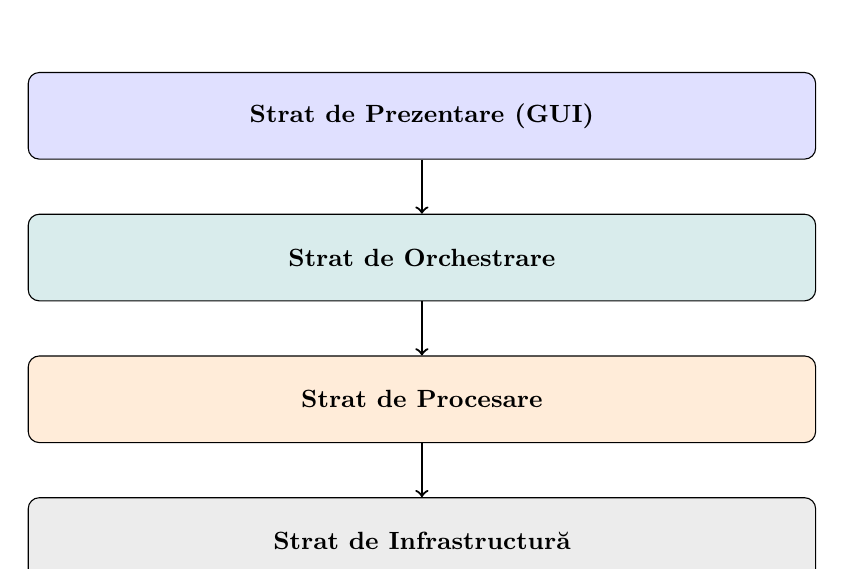
\begin{tikzpicture}[
    layer/.style={
        draw, rounded corners=4pt,
        minimum width=10cm, minimum height=1.1cm,
        align=center, font=\small\bfseries
    },
    sublabel/.style={font=\footnotesize, text=gray}
]

\node[layer, fill=blue!12]   (gui)      at (0, 0)    {Strat de Prezentare (GUI)};
\node[layer, fill=teal!15]   (pipeline) at (0, -1.8)  {Strat de Orchestrare};
\node[layer, fill=orange!15] (core)     at (0, -3.6)  {Strat de Procesare};
\node[layer, fill=gray!15]   (infra)    at (0, -5.4)  {Strat de Infrastructură};

\draw[->, thick] (gui.south)      -- (pipeline.north);
\draw[->, thick] (pipeline.south) -- (core.north);
\draw[->, thick] (core.south)     -- (infra.north);

\end{tikzpicture}
\caption{Arhitectura pe straturi a aplicației. Dependențele sunt direcționate exclusiv de sus în jos.}
\label{fig:layers}
\end{figure}

\section{Fluxul de Date}

La pornirea sistemului, \texttt{MainWindow} încarcă configurația tipizată din \texttt{config.toml} printr-un apel la \texttt{AppConfig.load()}. Când utilizatorul apasă butonul \textit{START} din ecranul de vizualizare live, \texttt{SystemViewWidget} instanțiază un \texttt{DepthPipeline} și pornește firul de inferență. Acesta inițializează \texttt{ModelRegistry} (care, în funcție de profilul hardware, încarcă fie modelul PyTorch, fie fișierul HEF pentru Hailo), deschide camera prin \texttt{CameraFactory} și pornește firul de captură.

La fiecare cadru disponibil, pipeline-ul aplică corecția de distorsiune, rulează inferența pentru a obține harta de adâncime, detectează planul solului prin RANSAC vectorizat și construiește masca, planifică traiectoria prin A*, și împachetează toate rezultatele într-un obiect \texttt{FrameResult}. Acesta este transmis stratului de prezentare prin semnalul Qt \texttt{\_result\_signal}, unde \texttt{SystemViewWidget} aplică suprapunerile vizuale și actualizează widget-ul de afișare.

Utilizatorul poate modifica parametrii sistemului în orice moment prin ecranul \textit{Settings}, care scrie valorile actualizate înapoi în \texttt{config.toml} și semnalizează ferestrei principale să reîncarce configurația. Modificările intră în vigoare la următoarea pornire a pipeline-ului.

\chapter{Rezultate}
\label{chap:ch5}

În acest capitol se vor discuta și observa exemple din viața reală, atât exemple în care fiecare componentă lucrează corect, cât și situații în care un nod din pipeline a scos rezultate inexact pentru a evidenția atât parțile pozitive, cât si cele negative.

Dat fiind faptul că testarea sistemul bazat pe Raspberry Pi este dependent de un monitor, dispozitive periferice cum ar fi mouse și tastatură, dar și o sursă de curent ce poate livra 5.1 Volți cu 5 Amperi, combinație ce se găsește rar pe piață, colectarea de date este anevoiasă. Din acest motiv, pentru Raspberry Pi s-a testat un singur scenariu, care este comparat cu sistemul bazat pe platforma NVidia. În fiecare secțiune se va discuta atât platforma NVidia testat independent, cât și în comparație cu Raspberry Pi.

Pentru sectiunile: \ref{sec:ch5sec1}, \ref{sec:ch5sec2}, \ref{sec:ch5sec3}, testarea se va face strict din punct de vedere vizual, bazat pe imagini din timpul rulării. Pentru ultima secțiune se vor compara date metrice. 

\section{Aproximarea Adâncimii}
\label{sec:ch5sec1}

Imaginile captate au fost realizate în urma unui proces în care s-a aplicat un filtru inferno asupra hărții de adâncimi, în care punctele apropiate au fost colorate închis, iar cele indepartate în culori aprinse. 

În timpul testării platformei bazată pe NVidia, s-a constat că aproximarea adâncimilor este realizată cu succes, în diverse scenarii, atât interioare cât și exterioare. În următoarele exemple se pot observa următoarele rezultatele vizuale: \ref{fig:exterior_estimare}, \ref{fig:interior_estimare}.

\begin{figure}[htbp]
    \centering
    % Prima imagine (stânga)
    \begin{minipage}{0.48\textwidth}
        \centering
        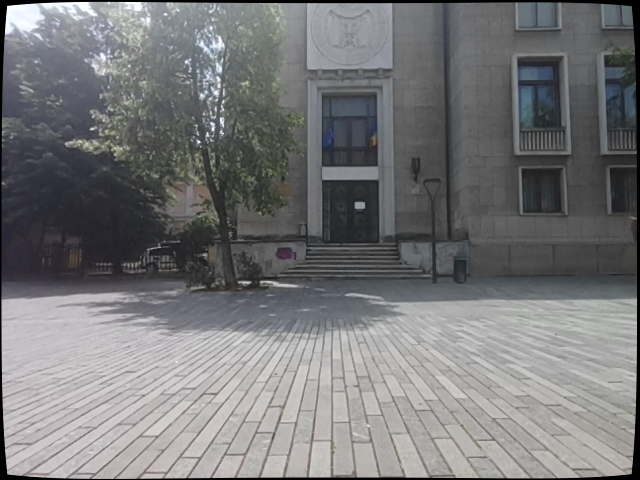
\includegraphics[width=\linewidth]{figures/real_world_examples/nvidia/20260604_114449_1_original.png}
        \caption{Imagine exteriroară captată după aplicării corecției.}
        \label{fig:exterior_original}
    \end{minipage}
    \hfill % Adaugă spațiu elastic între cele două imagini
    % A doua imagine (dreapta)
    \begin{minipage}{0.48\textwidth}
        \centering
        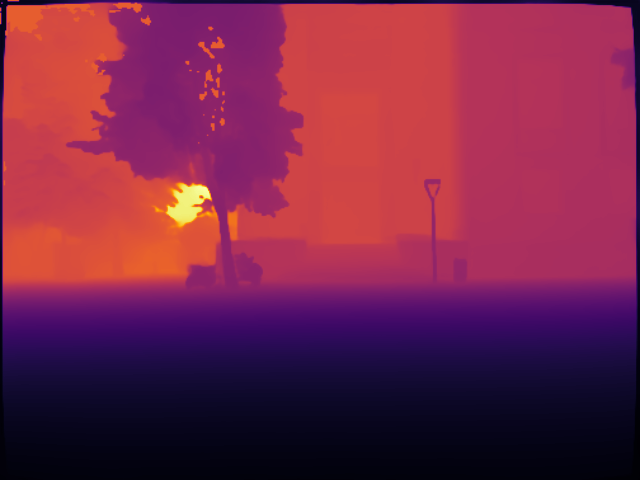
\includegraphics[width=\linewidth]{figures/real_world_examples/nvidia/20260604_114449_2_depth.png} % Schimbă cu numele imaginii tale
        \caption{Aproxamiare a adâncimi bazată pe imagine.}
        \label{fig:exterior_depth}
    \end{minipage}
    \caption{Comparație între imaginea orginilă și matricea de adâncime într-un scenariu exterior.}
    \label{fig:exterior_estimare}
\end{figure}

\begin{figure}[htbp]
    \centering
    % Prima imagine (stânga)
    \begin{minipage}{0.48\textwidth}
        \centering
        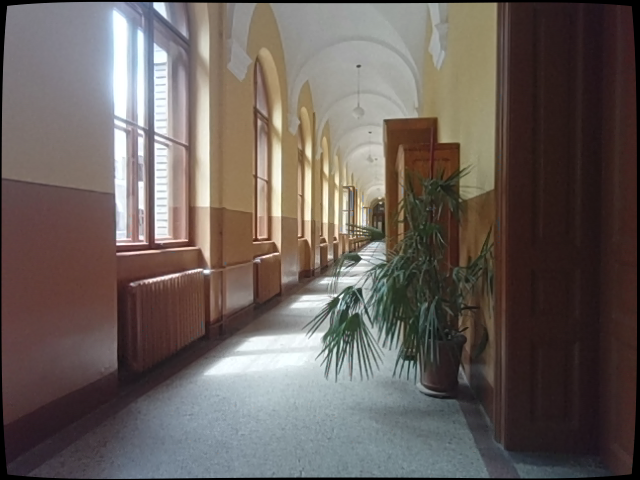
\includegraphics[width=\linewidth]{figures/real_world_examples/nvidia/20260604_115839_1_original.png}
        \caption{Imagine interioară captată după aplicării corecției.}
        \label{fig:interior_original}
    \end{minipage}
    \hfill % Adaugă spațiu elastic între cele două imagini
    % A doua imagine (dreapta)
    \begin{minipage}{0.48\textwidth}
        \centering
        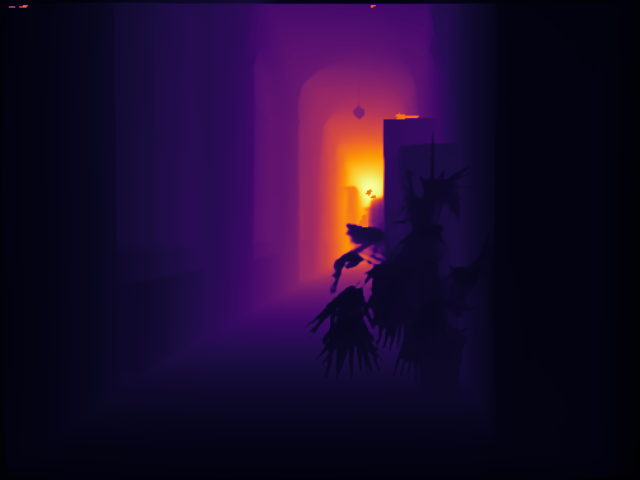
\includegraphics[width=\linewidth]{figures/real_world_examples/nvidia/20260604_115839_2_depth.png} % Schimbă cu numele imaginii tale
        \caption{Aproxamiare a adâncimi bazată pe imagine.}
        \label{fig:interior_depth}
    \end{minipage}
    \caption{Comparație între imaginea orginilă și matricea de adâncime într-un scenariu interior.}
    \label{fig:interior_estimare}
\end{figure}

Ținând cont că platforma bazată pe Raspberry Pi este limitată în putere, și modelul este atât cu o generație mai slab, cât și numărul de parametrii este mai mic, ne aștăm ca rezultatele sa fie mai slabe, și ele întradevăr sunt, dar mai degrabă când vine vorba de previzia muchiilor. Comparând matricea estimării cu imaginea orginilă se pot remarca elementele pe care le-a destins \ref{fig:interior_estimare_rpi}.

\begin{figure}[htbp]
    \centering
    % Prima imagine (stânga)
    \begin{minipage}{0.48\textwidth}
        \centering
        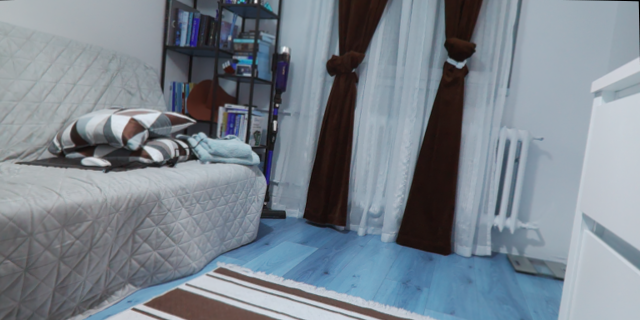
\includegraphics[width=\linewidth]{figures/real_world_examples/rpi/20260608_224242_1_original.png}
        \caption{Imagine interioară captată după aplicării corecției folosind Raspberry Pi + Hailo-8.}
        \label{fig:interior_original_rpi}
    \end{minipage}
    \hfill % Adaugă spațiu elastic între cele două imagini
    % A doua imagine (dreapta)
    \begin{minipage}{0.48\textwidth}
        \centering
        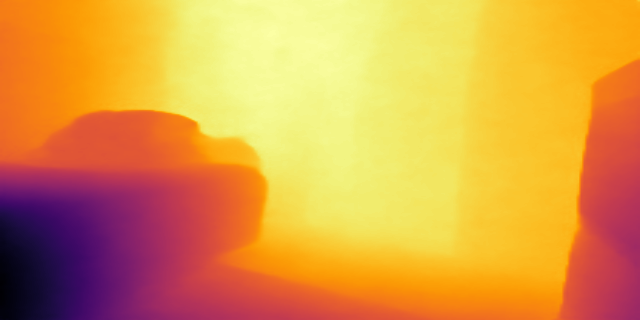
\includegraphics[width=\linewidth]{figures/real_world_examples/rpi/20260608_224242_2_depth.png} % Schimbă cu numele imaginii tale
        \caption{Aproxamiare a adâncimi bazată pe imagine folosind Raspberry Pi + Hailo-8.}
        \label{fig:interior_depth_rpi}
    \end{minipage}
    \caption{Comparație între imaginea orginilă și matricea de adâncime într-un scenariu interior folosind Raspberry Pi + Hailo-8.}
    \label{fig:interior_estimare_rpi}
\end{figure}

\section{Detecția Solului}
\label{sec:ch5sec2}

În majoritatea cazurile, detecția solului determină planul bine așa cum se poate vedea în figura \ref{fig:good_example_sol}.

\begin{figure}[htbp]
    \centering
    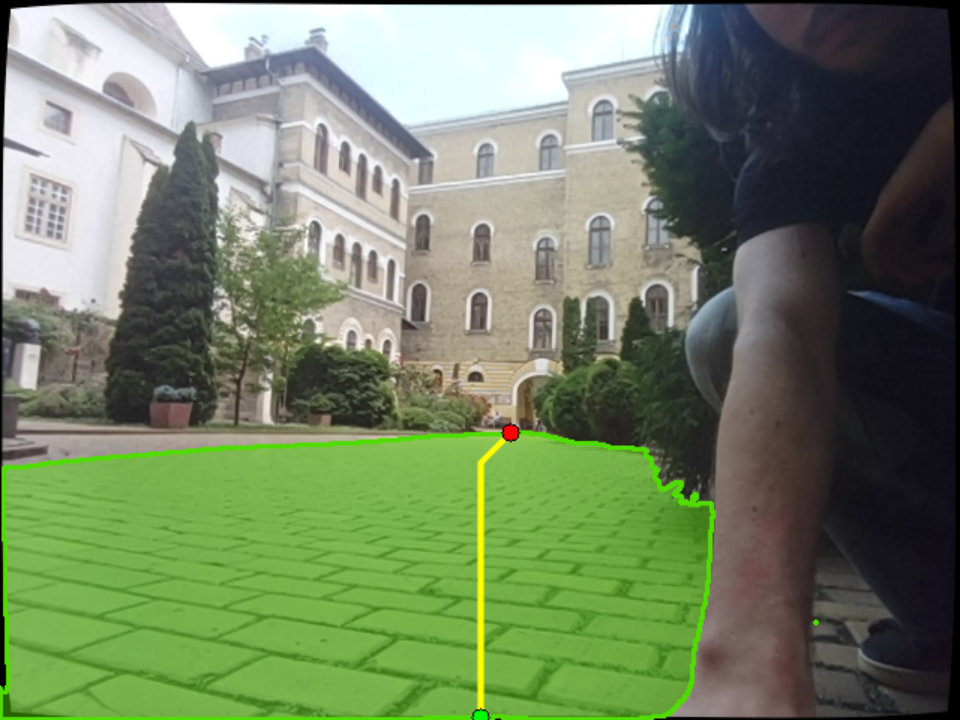
\includegraphics[width=0.8\linewidth]{figures/real_world_examples/nvidia/20260604_115437_5_view.png}
    \caption{Exemplu în care detecția solului detectează solul așa cum ne așteptăm.}
    \label{fig:good_example_sol}
\end{figure}

Cu toate acestea, s-a observat că pe traseele lungi nu sunt cuprinse în totalitatea, însemnând că sistemul nu detectează punctele distante ca facând parte din planul detectat al solului \ref{fig:long_road_example_sol}. Este greu de găsit un o explicație pentru acest fenomen, întrucât matricea adâncimi, din punct de vedere vizual, pare precisă așa cum se poate vedea în figura \ref{fig:long_road_example_sol_depth}. Mai multe studii pe acest fenomen trebuie efectuate.

\begin{figure}[htbp]
    \centering
    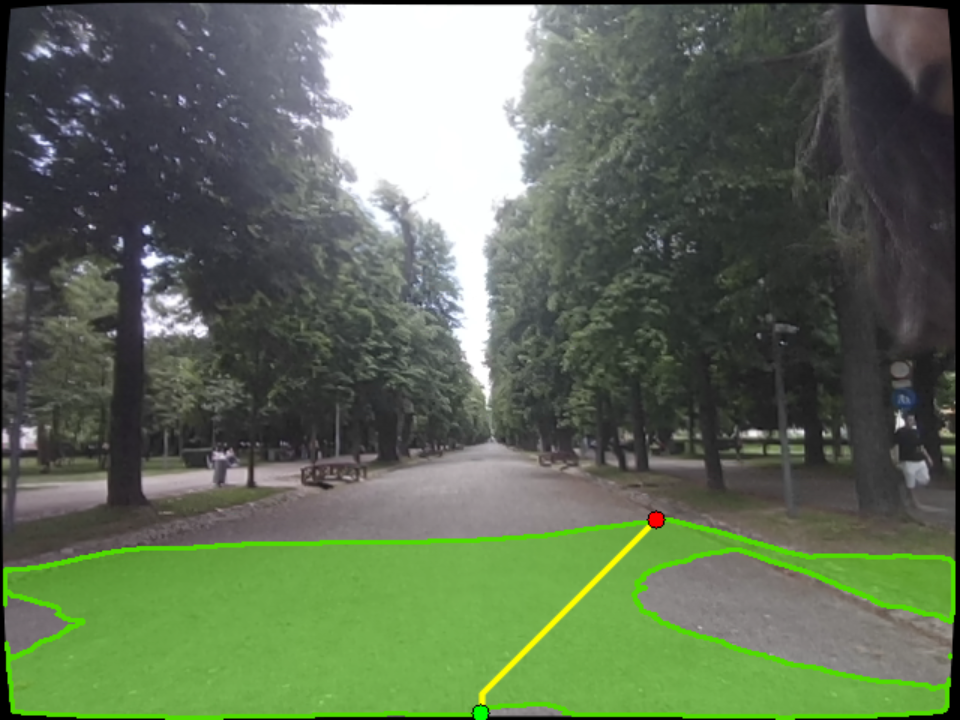
\includegraphics[width=0.8\linewidth]{figures/real_world_examples/nvidia/20260604_125553_5_view.png}
    \caption{Exemplu în care detecția solului nu detectează solul în totalitate.}
    \label{fig:long_road_example_sol}
\end{figure}

\begin{figure}[htbp]
    \centering
    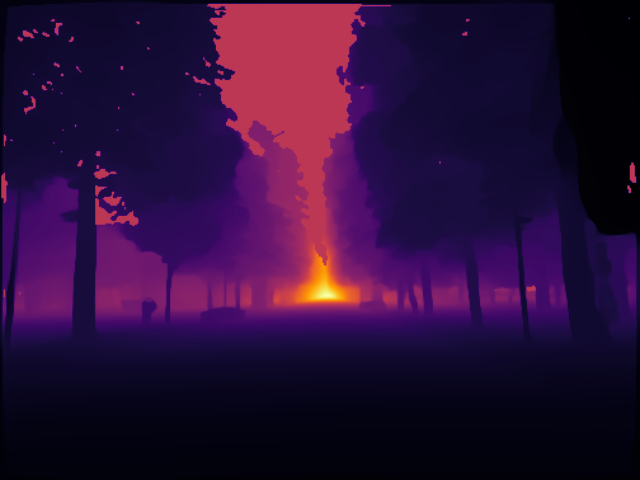
\includegraphics[width=0.8\linewidth]{figures/real_world_examples/nvidia/20260604_125553_2_depth.png}
    \caption{Matricea adâncimii pentru exemplul anterior.}
    \label{fig:long_road_example_sol_depth}
\end{figure}

O limitare majoră a metodei de detecție a solului aleasă pentru acest sistem stă tocmai în natura metodei. Pe scurt, detectează planul în care majoritatea punctelor din matricea de adâncime se află. Statistic vorbind, în majoritatea cazurilor acel plan este planului solului, însă în spații înguste acest fapt nu se mai aplică, iar planul solului este detectat greșit, așa cum se poate vedea în figura \ref{fig:small_space_sol}.

\begin{figure}[htbp]
    \centering
    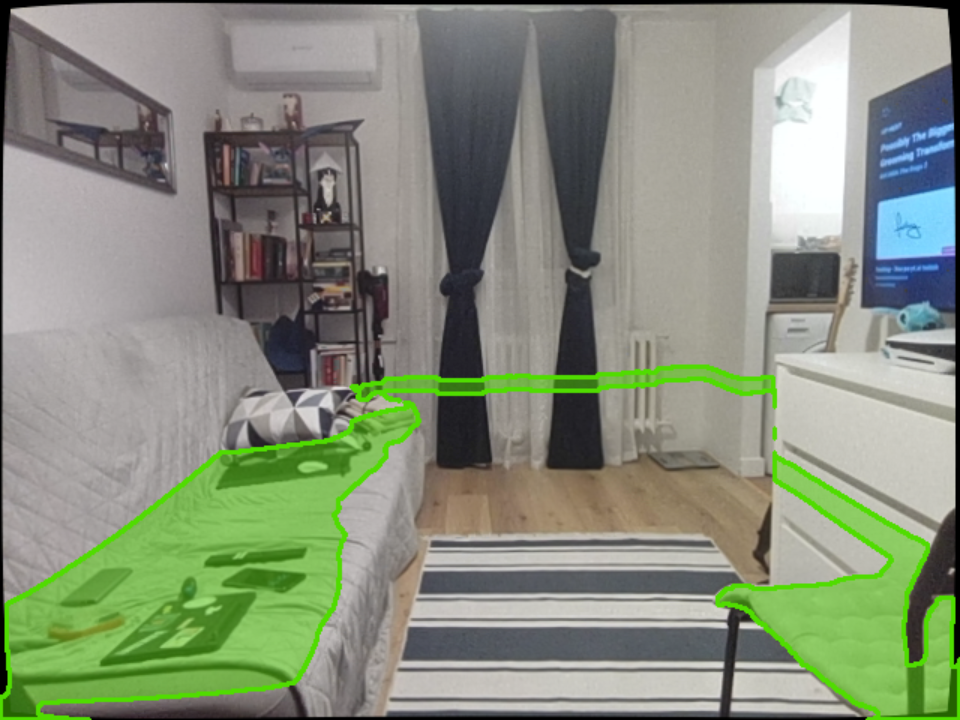
\includegraphics[width=0.8\linewidth]{figures/real_world_examples/nvidia/20260608_225109_5_view.png}
    \caption{Exemplu în care planul solului este detectat greșit datorită spațiului îngust.}
    \label{fig:small_space_sol}
\end{figure}

Totodată, s-a observat că în unele situații, sistemul detectează planul de mers cu porțiuni goale \ref{fig:spatii_sol}. Această problemă poate fi atribuită matricii de adâncime. 

\begin{figure}[htbp]
    \centering
    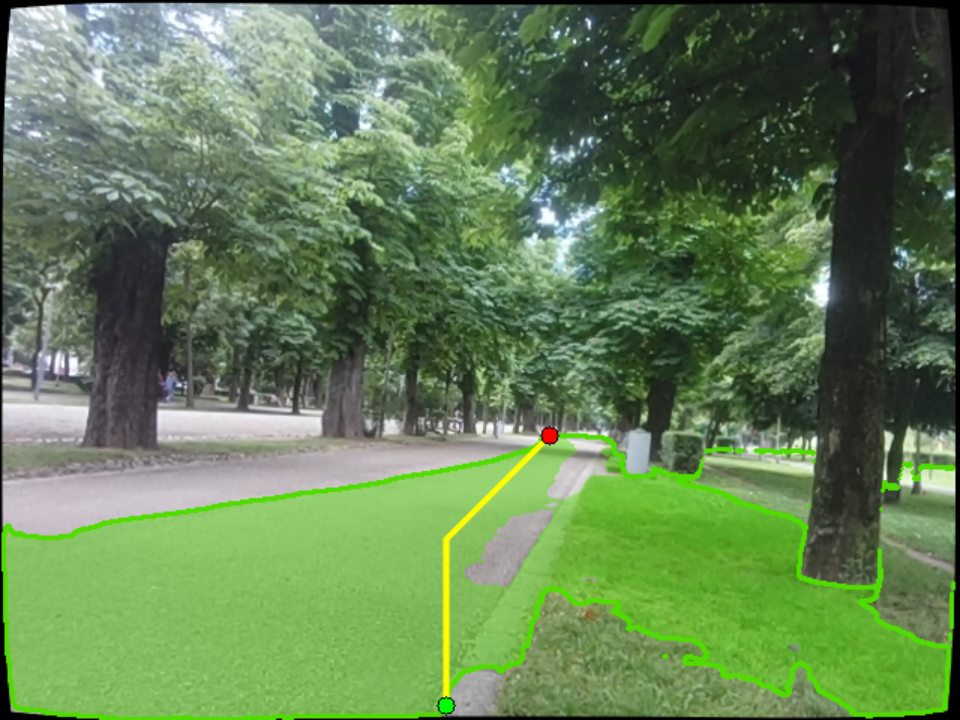
\includegraphics[width=0.8\linewidth]{figures/real_world_examples/nvidia/20260604_125945_5_view.png}
    \caption{Exemplu în care planul solului nu este detectat în întregime.}
    \label{fig:spatii_sol}
\end{figure}

Până în acest moment, toate aceste exemple au fost bazate de sistemul bazat pe NVidia. Comparând sistemul bazat pe nvidia vs. Raspberry Pi, se poate observa cum calitatea și precizia matricii de adâncimi influențează detecția solului, întrucât Raspberry Pi nu a reușit să detecteze solul precis, așa cum se poate vedea în figura \ref{}.

\begin{figure}[htbp]
    \centering
    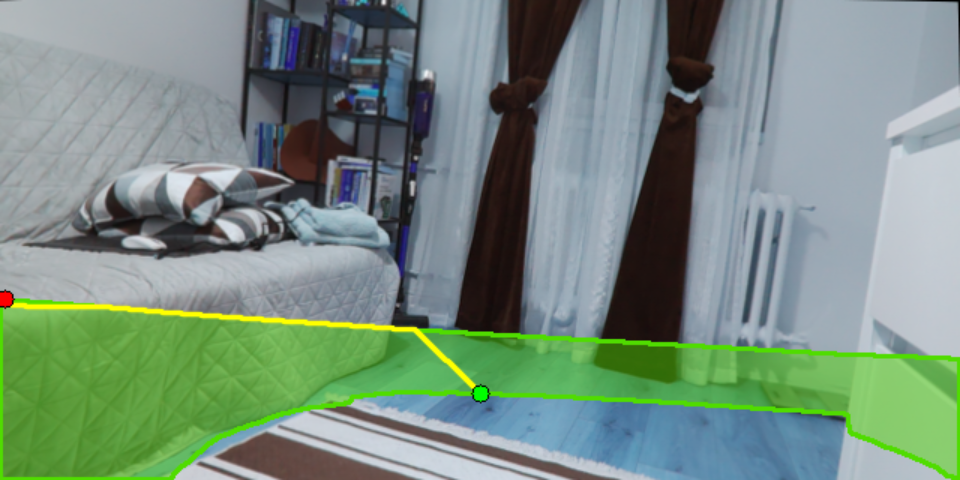
\includegraphics[width=0.8\linewidth]{figures/real_world_examples/rpi/20260608_224242_5_view.png}
    \caption{Exemplu în care Raspberry Pi-ul eșuează în a detecta solul.}
    \label{fig:rpi_sol}
\end{figure}

O altă limitare majoră este faptul că nu face distincția dintre un trotuar și o stradă circulată de mașini. Această metodă de determinare a solului a fost aleasă datorită vitezei de precosare superioară comparată cu metodele ce folosesc rețele neuronale, dat fiind scopul inițial de a construi un sistem compact, cu un buget relativ mic, și limitări hardware semnificative.

\section{Determinarea Drumului de Cost Minim}
\label{sec:ch5sec3}

Drumul de cost minim nu este găsit pe proiecția în 3D a planului de mers, dar mai bine zis pe proiecția lui în 2D. Acest lucru nu garantează că mereu se va găsi drumul de cost minim din viața reală, însă de cele mai multe ori este suficient.

\section{Latență}
\label{sec:ch5sec4}

Spre deosebire de secțiunile anterioare, evaluarea latenței se bazează pe date metrice colectate de modulul de profilare integrat în aplicație. Acesta măsoară, cu ajutorul funcției \texttt{time.perf\_counter()}, durata fiecărei etape a pipeline-ului pentru fiecare cadru procesat și o înregistrează într-un fișier CSV, în loturi, pentru a nu introduce întârzieri suplimentare pe calea critică. Statisticile prezentate în continuare au fost obținute pe platforma bazată pe NVidia (rezoluție 640$\times$480, model Depth Anything 3 metric, varianta Large), agregând aproximativ 9.989 de cadre din 13 sesiuni de rulare distincte. Primul cadru al fiecărei sesiuni a fost exclus, întrucât include inițializarea modelului și nu reflectă regimul normal de funcționare.

Pipeline-ul este compus din patru etape sincrone — corecția distorsiunii, estimarea adâncimii, detecția solului și determinarea drumului — a căror sumă constituie timpul total de procesare per cadru. Capturarea cadrului de la cameră se desfășoară pe un thread separat, în paralel cu procesarea, motiv pentru care nu este inclusă în timpul total, deși este raportată informativ. Rezultatele agregate sunt prezentate în tabelul \ref{tab:latenta_nvidia}.

\begin{table}[htbp]
    \centering
    \begin{tabular}{lcccc}
        \toprule
        Etapă & Medie & Mediană & Dev. std. & p95 \\
              & [ms] & [ms] & [ms] & [ms] \\
        \midrule
        Capturare cadru$^{*}$ & 34,1 & 32,1 & 4,0 & 42,4 \\
        Corecția distorsiunii & 0,5 & 0,5 & 1,7 & 0,7 \\
        Estimarea adâncimii & 64,1 & 64,1 & 9,1 & 69,5 \\
        Detecția solului & 0,9 & 0,9 & 0,3 & 1,1 \\
        Determinarea drumului & 47,7 & 13,7 & 200,9 & 212,3 \\
        \midrule
        Total procesare & 113,2 & 79,6 & 200,9 & 276,6 \\
        \bottomrule
    \end{tabular}
    \caption{Statistici de latență per etapă pe platforma NVidia, agregate peste 9.989 de cadre din 13 sesiuni de rulare (cadrul de inițializare exclus). $^{*}$Capturarea cadrului se execută pe un thread separat și nu este inclusă în timpul total de procesare.}
    \label{tab:latenta_nvidia}
\end{table}

După cum se poate observa, estimarea adâncimii domină timpul de procesare, reprezentând aproximativ 56\% din total (64,1 ms în medie). Aceasta este, de altfel, singura etapă bazată pe o rețea neuronală și constituie gâtuirea (\textit{bottleneck}) sistemului, fiind totodată foarte stabilă, cu o deviație standard de doar 9,1 ms. Prin contrast, etapele pur geometrice — corecția distorsiunii și detecția solului — sunt neglijabile, fiecare sub 1 ms, fapt ce confirmă decizia de proiectare de a folosi o metodă bazată pe RANSAC pentru detecția solului în locul unei a doua rețele neuronale.

Etapa de determinare a drumului prezintă un comportament aparte: în mod tipic este ieftină (mediană de 13,7 ms), însă distribuția sa are o coadă grea — aproximativ 19\% dintre cadre depășesc 50 ms, iar în cazuri degenerate căutarea drumului poate dura câteva secunde. Acest fapt explică diferența semnificativă dintre medie (47,7 ms) și mediană și se reflectă în cei doi indicatori ai cadenței: pornind de la mediana timpului total (79,6 ms) sistemul atinge aproximativ \textbf{12,6 cadre pe secundă}, în timp ce media (113,2 ms) corespunde unei valori de aproximativ \textbf{8,8 cadre pe secundă}. În practică, sistemul funcționează tipic în jurul valorii de 12 FPS, vârfurile ocazionale ale etapei de determinare a drumului cauzând micro-blocaje punctuale.

Pe platforma NVidia, performanța temporală este așadar mărginită de modelul de estimare a adâncimii, restul componentelor adăugând un cost redus și predictibil. O eventuală optimizare a latenței ar trebui să vizeze în primul rând accelerarea inferenței modelului de adâncime și, secundar, stabilizarea etapei de determinare a drumului în cazurile nefavorabile.

Pentru a evidenția impactul platformei hardware asupra latenței, aceleași măsurători au fost realizate și pe sistemul bazat pe Raspberry Pi + Hailo-8. Spre deosebire de platforma NVidia, aici estimarea adâncimii este delegată acceleratorului neuronal Hailo-8 și folosește un model mult mai mic — Depth Anything 2, varianta ViT-S, la rezoluția 224$\times$224, în mod relativ. Statisticile, agregate peste aproximativ 2.086 de cadre din 2 sesiuni de rulare, sunt prezentate în tabelul \ref{tab:latenta_rpi}.

\begin{table}[htbp]
    \centering
    \begin{tabular}{lcccc}
        \toprule
        Etapă & Medie & Mediană & Dev. std. & p95 \\
              & [ms] & [ms] & [ms] & [ms] \\
        \midrule
        Capturare cadru$^{*}$ & 59,1 & 53,9 & 32,2 & 122,8 \\
        Corecția distorsiunii & 3,8 & 3,3 & 5,3 & 7,1 \\
        Estimarea adâncimii & 42,3 & 41,8 & 1,8 & 45,7 \\
        Detecția solului & 6,1 & 5,6 & 2,2 & 10,4 \\
        Determinarea drumului & 83,4 & 36,7 & 105,4 & 226,3 \\
        \midrule
        Total procesare & 135,5 & 90,8 & 104,8 & 277,7 \\
        \bottomrule
    \end{tabular}
    \caption{Statistici de latență per etapă pe platforma Raspberry Pi + Hailo-8, agregate peste 2.086 de cadre din 2 sesiuni de rulare (cadrul de inițializare exclus). $^{*}$Capturarea cadrului se execută pe un thread separat și nu este inclusă în timpul total de procesare.}
    \label{tab:latenta_rpi}
\end{table}

Rezultatele relevă o inversare a profilului de latență față de platforma NVidia. Dacă acolo gâtuirea o constituia estimarea adâncimii, pe Raspberry Pi această etapă devine una dintre cele mai rapide (42,3 ms în medie, sub valoarea de pe NVidia și remarcabil de stabilă, cu o deviație standard de doar 1,8 ms), tocmai datorită modelului mult mai mic rulat pe NPU-ul dedicat. În schimb, gâtuirea se mută pe etapa de determinare a drumului (83,4 ms în medie, aproximativ 61\% din total), care se execută pe procesorul ARM, semnificativ mai lent decât GPU-ul plăcii NVidia. Această etapă prezintă din nou o coadă grea, peste 43\% dintre cadre depășind 50 ms. Trebuie subliniat însă că latențele estimării adâncimii nu sunt direct comparabile din punct de vedere calitativ, întrucât cele două platforme rulează modele diferite ca generație și dimensiune, așa cum s-a discutat în secțiunea \ref{sec:ch5sec1}.

În ansamblu, cele două platforme ating cadențe surprinzător de apropiate — aproximativ 11,0 cadre pe secundă (mediană) pe Raspberry Pi față de 12,6 pe NVidia — însă din motive diferite: sistemul NVidia este mărginit de inferența unui model de adâncime puternic, în timp ce sistemul Raspberry Pi, deși descarcă inferența pe NPU, este mărginit de calculele geometrice efectuate pe procesorul ARM. Această observație sugerează că, pe platforma embedded, optimizarea ar trebui să vizeze în primul rând etapa de determinare a drumului, complementar față de direcția indicată pentru platforma NVidia.


\chapter{Direcții viitoare și Concluzii}
%\chapter*{Concluzii}
\label{conclusions}

\par Concluzii ...

%\addcontentsline{toc}{chapter}{Concluzii}
%\addcontentsline{toc}{chapter}{Conclusions}

\bibliography{references}

\end{document}
